%%%
%
% $Autor: Wings $
% $Datum: 2023-03-01 $
% $Dateiname: IMULibFunctions$
% $Version: 1 $
%
%%%


\chapter{IMU LSM6DSOX - Libraries and Functions}  \label{Chap: Libraries and Functions}

\section{Libraries}

A library refers to a collection of pre-written code that can be used by developers to perform specific tasks or functions without having to write the code from scratch. Libraries are designed to make the development process easier and more efficient by providing pre-built solutions to common programming challenges.

\subsection{Wire.h}
Wire.h is a library in Arduino that allows for communication between I2C devices. I2C stands for Inter-Integrated Circuit, which is a synchronous serial communication protocol used for connecting microcontrollers to peripheral devices. Wire.h provides functions for initializing the I2C bus, sending and receiving data over the bus, and managing multiple devices on the same bus. With this library, developers can easily connect multiple I2C devices, such as sensors or displays, to an Arduino board.\cite{arduinoLCDI2C:2023,Aristi:2021}

\subsection{Kalman.h}
Kalman.h is a library that implements the Kalman filter algorithm. The Kalman filter is a mathematical technique used to estimate the state of a system based on incomplete measurements. It is commonly used in control systems, robotics, and navigation applications to improve the accuracy of sensor measurements and reduce errors. Kalman.h provides a simple interface for developers to implement the Kalman filter in their Arduino projects.\cite{arduino:2019Kalman,Fetick:2021}

\subsection{Arduino\_LSM6DSOX.h}
Arduino\_LSM6DSOX.h is a library that provides access to the LSM6DSOX accelerometer and gyroscope sensor on the Arduino Mbed OS Nicla Board. The LSM6DSOX sensor is a 6-axis sensor that can measure both linear acceleration and angular velocity. Arduino\_LSM6DSOX.h provides functions for initializing the sensor, reading data from the sensor, and configuring the sensor parameters. With this library, developers can easily integrate the LSM6DSOX sensor into their Arduino projects and use the sensor data for various applications, such as gesture recognition or orientation detection.\cite{arduino:2021lsm6dsox}

\subsection{LSM6DSOXSensor.h}

\FILE{LSM6DSOXSensor.h} is a library that provides an interface for interacting with the LSM6DSOX sensor. The LSM6DSOX is a 6-axis inertial measurement unit (IMU) sensor that combines a 3-axis accelerometer and a 3-axis gyroscope in a single chip. It is commonly used in applications that require motion sensing and orientation tracking, such as robotics, drones, wearable devices, and Internet of Things (IoT) devices.The LSM6DSOXSensor.h library allows developers to easily interact with the LSM6DSOX sensor by providing functions and classes for configuring the sensor, reading raw sensor data, and performing sensor fusion to obtain calibrated accelerometer and gyroscope data, as well as derived data such as orientation, linear acceleration, and angular velocity. The library abstracts the low-level communication with the sensor, providing a higher-level API that simplifies the process of working with the sensor.



\section{Functions}
A function is a block of code that performs a specific task or set of tasks. Functions are designed to be reusable and modular, meaning they can be called and executed multiple times throughout a program without having to rewrite the code every time. Functions can take input parameters, perform operations on them, and return output values.


\subsection{setup()}
The setup() function is a special function in the Arduino programming language that is called once at the beginning of the program. The purpose of the setup() function is to initialize variables, pin modes, and other settings that are necessary for the program to run correctly. This function is typically used to set up hardware components, such as sensors or displays, and configure any necessary settings, such as communication protocols or data rates.\cite{ArduinoSetup:2019}

\subsection{loop()}
The loop() function is another special function in the Arduino programming language that is called repeatedly after the setup() function. The purpose of the loop() function is to execute the main code of the program in a continuous loop until the program is terminated. This function is typically used to read sensor data, perform calculations, and control hardware components based on the input data.\cite{ArduinoLoop:2019}

\subsection{IMU.begin()}
IMU.begin() is a function provided by the Arduino\_LSM6DSOX.h library, which is used to initialize the LSM6DSOX accelerometer and gyroscope sensor on the Arduino Mbed OS Nicla Board. The purpose of the IMU.begin() function is to set up the communication between the Arduino board and the LSM6DSOX sensor and to configure the sensor settings to match the requirements of the program. This function is typically called in the setup() function of the program to initialize the sensor before reading data from it in the loop() function.

\subsection{IMU.setAccelerometerRange()}
The IMU.setAccelerometerRange() function is used to set the range of the accelerometer on the LSM6DSOX sensor. The accelerometer range determines the maximum acceleration that can be measured by the sensor. This function takes an argument that specifies the range in Gs (gravitational force) and can be set to 2G, 4G, 8G, or 16G depending on the application requirements.

\subsection{IMU.setGyroscopeRange()}
The IMU.setGyroscopeRange() function is used to set the range of the gyroscope on the LSM6DSOX sensor. The gyroscope range determines the maximum angular velocity that can be measured by the sensor. This function takes an argument that specifies the range in degrees per second (dps) and can be set to 125dps, 250dps, 500dps, 1000dps, or 2000dps depending on the application requirements.

\subsection{IMU.setAccelerometerDataRate()}
The IMU.setAccelerometerDataRate() function is used to set the data rate of the accelerometer on the LSM6DSOX sensor. The data rate determines how often the sensor samples the acceleration data and can be set to 12.5Hz, 26Hz, 52Hz, 104Hz, 208Hz, 416Hz, 833Hz, or 1660Hz depending on the application requirements.

\subsection{IMU.setGyroscopeDataRate()}
The IMU.setGyroscopeDataRate() function is used to set the data rate of the gyroscope on the LSM6DSOX sensor. The data rate determines how often the sensor samples the angular velocity data and can be set to 12.5Hz, 26Hz, 52Hz, 104Hz, 208Hz, 416Hz, 833Hz, or 1660Hz depending on the application requirements.

\subsection{IMU.accelerationSampleRate()}
The IMU.accelerationSampleRate() function is used to read the current sample rate of the accelerometer on the LSM6DSOX sensor. This function returns the current data rate value in Hz.

\subsection{IMU.gyroscopeSampleRate()}
The IMU.gyroscopeSampleRate() function is used to read the current sample rate of the gyroscope on the LSM6DSOX sensor. This function returns the current data rate value in Hz.

\subsection{IMU.temperatureAvailable()}
The IMU.temperatureAvailable() function is provided by the Arduino\_LSM6DSOX.h library for the LSM6DSOX accelerometer and gyroscope sensor on the Arduino Mbed OS Nicla Board. This function is used to check if the temperature data is available to be read from the sensor. It returns a boolean value of true if the temperature data is available, and false if it is not.

\subsection{IMU.readTemperature()}
The IMU.readTemperature() function is provided by the Arduino\_LSM6DSOX.h library and is used to read the temperature data from the LSM6DSOX sensor on the Arduino Mbed OS Nicla Board. This function returns the temperature in degrees Celsius as a floating-point value. Before calling this function, you should use the temperatureAvailable() function to check if the temperature data is available.

\subsection{IMU.accelerationAvailable()}
The IMU.accelerationAvailable() function is provided by the Arduino\_LSM6DSOX.h library and is used to check if the acceleration data is available to be read from the LSM6DSOX sensor on the Arduino Mbed OS Nicla Board. It returns a boolean value of true if the acceleration data is available, and false if it is not.

\subsection{IMU.readAcceleration()}
The IMU.readAcceleration() function is provided by the Arduino\_LSM6DSOX.h library and is used to read the acceleration data from the LSM6DSOX sensor on the Arduino Mbed OS Nicla Board. This function returns a 3D vector that represents the acceleration in units of Gs (gravitational force) along the x, y, and z axes. Before calling this function, you should use the accelerationAvailable() function to check if the acceleration data is available.

\subsection{IMU.gyroscopeAvailable()}
The IMU.gyroscopeAvailable() function is provided by the Arduino\_LSM6DSOX.h library and is used to check if the gyroscope data is available to be read from the LSM6DSOX sensor on the Arduino Mbed OS Nicla Board. It returns a boolean value of true if the gyroscope data is available, and false if it is not.

\subsection{IMU.readGyroscope()}
The IMU.readGyroscope() function is provided by the Arduino\_LSM6DSOX.h library and is used to read the gyroscope data from the LSM6DSOX sensor on the Arduino Mbed OS Nicla Board. This function returns a 3D vector that represents the angular velocity in units of degrees per second (dps) along the x, y, and z axes. Before calling this function, you should use the gyroscopeAvailable() function to check if the gyroscope data is available.

\subsection{randomGaussian() }
The randomGaussian() function is a built-in function in the Arduino programming language. Gaussian distribution is also known as normal distribution, and it is a probability distribution that describes how values are distributed around the mean. This function takes two arguments: the mean and the standard deviation of the distribution. It returns a random floating-point number with a mean value equal to the first argument and a standard deviation equal to the second argument. This function is commonly used in statistical simulations and signal-processing application.

\subsection{kalmanX.setQ(), kalmanY.setQ(), kalmanZ.setQ()}
These functions set the process noise covariance for the Kalman filter in the X, Y, and Z axes respectively. The process noise covariance controls how much we trust our prediction of the state of the system at the next time step. A higher value of Q indicates that the system is more likely to deviate from the predicted state and a lower value indicates that the system is more likely to follow the predicted state.

\subsection{kalmanX.setR(), kalmanY.setR(), kalmanZ.setR() }
These functions set the measurement noise covariance for the Kalman filter in the X, Y, and Z axes respectively. The measurement noise covariance controls how much we trust the sensor measurement of the system. A higher value of R indicates that the sensor measurement is less reliable and a lower value indicates that the sensor measurement is more reliable.

\subsection{kalmanX.update(), kalmanY.update(), kalmanZ.update() }
These functions update the Kalman filter in the X, Y, and Z axes respectively. They take a measurement of the system and use it to update the state estimate of the system. The function returns the estimated bias of the measurement. The estimated bias is subtracted from the measurement to get a corrected measurement, which is used to update the state estimate.

\subsection{kalmanX.getSigma(), kalmanY.getSigma(), kalmanZ.getSigma() }
These functions return the standard deviation of the Kalman filter output in the X, Y, and Z axes respectively. The standard deviation is a measure of the noise in the output of the Kalman filter.

\subsection{delay() }
This function causes the program to pause execution for a specified number of milliseconds. In this code, it is used to wait for a short time before reading from the IMU again. This allows time for the IMU to take a new measurement and for the Kalman filter to update its estimates.

\subsection{lsm6dsoxSensor.Set\_X\_FS()}
lsm6dsoxSensor.Set\_X\_FS() is a function provided by the LSM6DSOXSensor.h library that is used to set the full-scale range of the accelerometer in the LSM6DSOX sensor. The accelerometer measures acceleration along three axes (X, Y, Z) and the full-scale range determines the maximum range of acceleration that the sensor can measure without saturation.

The function takes an argument that specifies the desired full-scale range for the accelerometer. The available options for the resolution range may vary depending on the specific sensor model, but commonly include ±2g, ±4g, ±8g, or ±16g. The full-scale range is typically expressed in units of acceleration (e.g., g) and represents the maximum acceleration that the sensor can accurately measure along each axis.

When lsm6dsoxSensor.Set\_X\_FS() is called with the desired resolution range as an argument, the function sends the appropriate configuration commands to the LSM6DSOX sensor to set the accelerometer to the specified full-scale range. This ensures that the sensor is configured to accurately measure accelerations within the desired range and prevents saturation of the sensor's output, which can result in inaccurate readings.

\subsection{lsm6dsoxSensor.Set\_G\_FS()}
lsm6dsoxSensor.Set\_G\_FS() is a method or function call that likely belongs to a software library or codebase that interfaces with an LSM6DSOX sensor. The LSM6DSOX is a type of inertial measurement unit (IMU) sensor that combines a 3-axis accelerometer and a 3-axis gyroscope in a single chip.

The Set\_G\_FS() function is likely used to configure the full-scale (FS) range or sensitivity of the gyroscope component of the LSM6DSOX sensor. Gyroscopes measure angular velocity or rotational motion, and the full-scale range determines the maximum angular velocity that the gyroscope can accurately measure.

The full-scale range is typically specified in units of degrees per second (dps) or radians per second (rad/s) and represents the maximum rate of rotation that the gyroscope can detect without saturating its output. A higher full-scale range allows the gyroscope to measure faster rotations, but it may result in reduced resolution for slower rotations.

The Set\_G\_FS() function likely takes an argument or parameter that specifies the desired full-scale range for the gyroscope, such as +/- 125 dps, +/- 250 dps, +/- 500 dps, +/- 1000 dps, or +/- 2000 dps, depending on the capabilities of the LSM6DSOX sensor. The function would then configure the sensor to operate with the specified full-scale range for the gyroscope accordingly

\subsection{Initialize\_IMU()}
The Initialize\_IMU() function is responsible for initializing and configuring the LSM6DSOX sensor for operation. It begins by establishing communication with the sensor using the Wire.begin() function, which is commonly used for I2C communication in Arduino-based projects. Next, it initializes the LSM6DSOX sensor using the lsm6dsoxSensor.begin() function, which sets up the sensor for operation.

The function then proceeds to set the full-scale range for the accelerometer and gyroscope using the lsm6dsoxSensor.Set\_X\_FS() and lsm6dsoxSensor.Set\_G\_FS() functions, respectively. In this case, the full-scale range is set to ±4g for the accelerometer and ±2000 deg/s for the gyroscope, which determines the maximum range of motion that the sensor can measure.

The sample rates for both the accelerometer and gyroscope are then set to 104 Hz using the lsm6dsoxSensor.Set\_X\_ODR() and lsm6dsoxSensor.Se\_G\_ODR() functions, respectively. The sample rate determines how frequently the sensor measures and reports data, with a higher sample rate resulting in more frequent updates but potentially higher power consumption.

\subsection{Factors\_Calculation()}
The Factors\_Calculation() function performs several steps. First, it checks if temperature data is available from the IMU sensor using the IMU.temperatureAvailable() function. If temperature data is available, it reads the temperature readings from the IMU using the IMU.readTemperature() function and stores the value in the temperature variable. Then, it calculates the temperature factor by multiplying the temperature sensitivity, temperature, and temperature tolerance, and dividing the result by 100.0 to convert the tolerance from percentage to decimal. Next, it calculates the linear acceleration factor by multiplying the linear acceleration sensitivity and linear acceleration tolerance. Finally, it calculates the angular rate factor by multiplying the angular rate sensitivity and angular rate tolerance.

\subsection{Factors\_Calculation()}
The Accelerometer\_Gyroscope\_Characteristics() function performs several steps. First, it checks if accelerometer data is available from the IMU sensor using the IMU.accelerationAvailable() function. If accelerometer data is available, it reads the accelerometer readings for the X, Y, and Z axes from the IMU using the IMU.readAcceleration() function and stores the values in the variables Ax, Ay, and Az. Then, it calculates the acceleration in m/s\^2 for each axis by multiplying the raw accelerometer readings with the linear acceleration factor, temperature factor, and gravity. The calculated values are stored in the variables Ax\_m\_sec2, Ay\_m\_sec2, and Az\_m\_sec2. Next, it adds noise characteristics to the accelerometer readings by calculating the noise values for each axis based on the accelerometer noise density and sample rate, and then adding them to the corresponding calculated acceleration values. It also checks if gyroscope data is available from the IMU sensor using the IMU.gyroscopeAvailable() function. If gyroscope data is available, it reads the gyroscope readings for the X, Y, and Z axes from the IMU using the IMU.readGyroscope() function and stores the values in the variables Gx, Gy, and Gz. Finally, it converts the gyroscope readings from LSB to deg/s by multiplying with the angular rate factor and temperature factor, and stores the calculated values in the variables Gx\_deg\_sec, Gy\_deg\_sec, and Gz\_deg\_sec.

\chapter{Sensor Inertial Mesure Unit}

Inertial Measurement Units (IMU) are an component of many navigation and control systems. These devices integrate several sensors, including accelerometers and gyroscopes, to measure and foolow an object's, linear and rotationnal, movements in three-dimensional space. IMUs are widely used in a variety of applications, such as autonomous vehicle navigation, virtual reality, image stabilization, and even in wearable devices for tracking physical activity. Their ability to provide precise data on linear and angular acceleration makes them indispensable tools for systems requiring precise control and orientation, and ongoing technological advances have reduced their size, power consumption and cost, widening their scope of application in many fields. \cite{STMicroelectronics:2015}


\section{General Description }

The Inertial Mesure Unit is used to mesured acceleration or rotation motion, this is an electronic devise who used  3 types of sensors :  magnetometer, accelerometer and gyroscope. 
This IMU used sensor LSM9DS1 and they give velocity, orientation and gravital force. 

The magnetometer can mesured the strenght of magnetic fields, this mesure can give different information, if you pass a current through an electromagnet or in any other way.

\subsection{Always On Mode}

This feature implies that the LSM9DS1 can remain operational continuously, even when a device is in sleep mode, without excessively draining power. Such functionality proves invaluable for applications demanding uninterrupted motion tracking, like fitness monitoring or navigation systems.

\bigskip

The power consumption is an important factor when we have battery-powered device like smartphone or other portable application.  This device is portable, so they need less battery than possible to do less weight than possible. 

\bigskip

The LSM9DS1 boasts a power consumption of 0.55 mA when operating in combo high-performance mode. This signifies its ability to maintain a low power consumption level while delivering exceptional data quality. In this mode, the sensor excels in concurrently measuring acceleration and angular rate, ensuring precise and reliable data output even at a high sampling rate.


\subsection{Tilt detection}

The Tilt detection detect movement with accelerometer, if movement is doing so Tilt detect it. Tilt function with Ultra Low Power consumption. 

Per example, if you have your smartphone in your front pant poket. Tilt detection can sayed if you standing to sitting or sitting to standing.

\subsection{Significant Motion Detection}

The Significant Motion Detection used in LSM9DS1 only accelerometer to detect big movement. It can used for different usage : 
\begin{itemize}
    \item Waking up a device from sleep mode when the user starts moving.
    \item Tracking steps or activity changes in fitness applications.
    \item Triggering alarms or notifications when a significant movement is detected.
\end{itemize}

\section{Specific Sensor }
\subsection{LSM9DS1}

The sensor LSM9DS1, engineered by STMicroelectronics, is composed of a 3-axis Inertial Measurement Unit (IMU), who have a high-performance 3-axis digital accelerometer and 3-axis digital gyroscope. This device is meticulously crafted for precise motion follow up, finding widespread application in wearable devices and smartphones. Capable of concurrent measurement of both linear and rotational motion, it stands as a hallmark in motion-sensing technology.

The sensor LSM9DS1 was devellop to detect movement, stationary/motion detection, tilt, pedometer functions, timestamping and to support the data and acquisition of an external magnetometer. This sensor give hardware flexibility to connect the pins with different mode connections to external sensors to expand functionalities such as adding a sensor hub, auxiliary SPI.

\bigskip

\subsection{Accelerometer}

The STMicroelectronics LSM9DS1 accelerometer is a  sensor designed to measure linear acceleration along the x, y, and z-axes. With a typical measurement range of ±2g, ±4g,±8g,±16g. It's give  precision and reliability for a variety of applications.The accelerometer for LSM9DS1  has an acceleration sampling frequency that can be changed to the following values: 10 Hz, 50 Hz, 119 Hz, 238 Hz, 476 Hz, 952 Hz.

\bigskip

It's low power consumption makes it an great choice for battery-powered devices, with a typical operating current ranging from 0.55 mA to 1.25 mA. Additionally, it's wide operating voltage range, from 1.71 V to 3.6 V, allows it to easily adapt to different system configurations.

\bigskip

Whether it's tracking movements in wearable devices, stabilizing drones, or measuring vibrations in structures, the accelerometer LSM9DS1 delivers outstanding performance in a compact and robust package.

The STMicroelectronics accelerometer LSM9DS1 is a preferred choice for engineers and designers seeking a precise and reliable solution for their projects.

\bigskip 

\begin{center}
    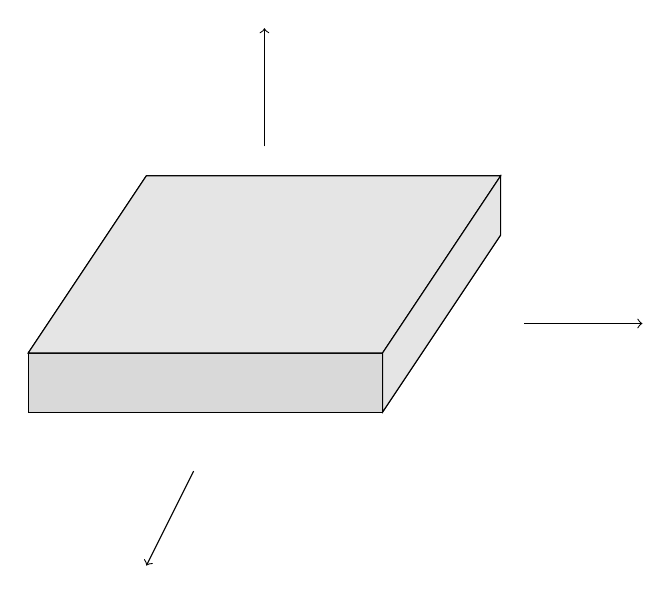
\begin{tikzpicture}[scale=1.5]
        % Face avant
        \draw[fill=gray!30] (0,0) rectangle (3,0.5);
        
        \draw (0,0.5) -- (1,2);
        \draw (3, 0.5) -- (4,2);
        \draw (3,0) -- (4,1.5);
        \draw (4,1.5) -- (4,2);
        \draw (1,2) -- (4,2);
        \draw[fill=gray!20] (0,0.5) -- (3,0.5) -- (4,2) -- (1,2) -- cycle;
        \draw[->] (2, 2.25) -- (2, 3.25);
        \draw[->] (4.2, 0.75) -- (5.2, 0.75);
        \draw[->] (1.4,- 0.5) -- (1,-1.3);
        \draw[fill=gray!20] (3,0) -- (3,0.5) -- (4,2) -- (4,1.5) -- cycle;			
    \end{tikzpicture}
    
    \captionof{figure}{LSM9DS1 axis  on this card}	
\end{center}

\subsection{Gyroscope}

The STMicroelectronics LSM9DS1 gyroscope is a  measuring instrument designed to assess rotation rates around the x, y, and z-axes. With a typical measurement range of ±245, ±500, ±2000 dps, it offers adaptability to the specific needs of the application.The gyroscope of LSM9DS1  has an acceleration sampling rate that can be modified to take the following values: 14.9 Hz, 59.5 Hz, 119 Hz, 238 Hz, 476 Hz, 952 Hz.
\bigskip

This gyroscope operates with a voltage range of 1.71 V to 3.6 V, allowing it to easily integrate into different system configurations. Furthermore, its typical operating current ranges from 1 mA to 2 mA, ensuring optimal energy efficiency for battery-powered devices.

\bigskip

Whether it's for inertial navigation, drone stabilization, or other applications requiring precise motion measurement, the gyroscope of LSM9DS1  delivers reliable and accurate performance in a compact and robust form factor, meeting the highest requirements of engineers and designers.

\begin{center}
    
    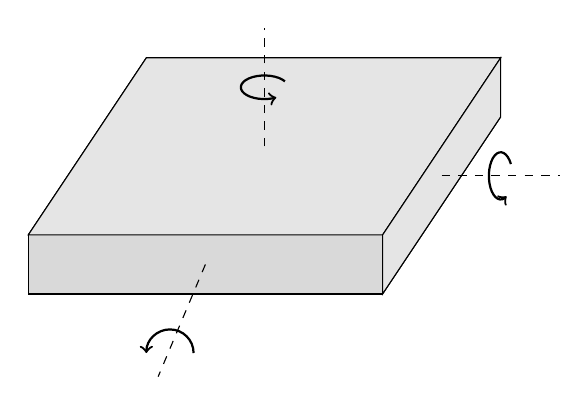
\begin{tikzpicture}[scale=1.5]
        % Face avant
        \draw[fill=gray!30] (0,0) rectangle (3,0.5);
        
        \draw (0,0.5) -- (1,2);
        \draw (3, 0.5) -- (4,2);
        \draw (3,0) -- (4,1.5);
        \draw (4,1.5) -- (4,2);
        \draw (1,2) -- (4,2);
        \draw[fill=gray!20] (0,0.5) -- (3,0.5) -- (4,2) -- (1,2) -- cycle;
        \draw[fill=gray!20] (3,0) -- (3,0.5) -- (4,2) -- (4,1.5) -- cycle;
        \draw[dashed] (2, 1.25) -- (2, 2.25);
        \draw[dashed] (3.5, 1) -- (4.5,1);
        \draw[dashed] (1.5,0.25) -- (1.1,-0.7);
        \draw[thick, ->] (1.4,-0.5) arc[start angle=0,end angle=180,radius=0.2];
        \draw [black, thick, domain=30:300, ->] plot ({2+0.2*cos(\x)}, {1.75+0.1*sin(\x)});
        \draw [black, thick, domain=30:300, ->] plot ({4+0.1*cos(\x)}, {1+0.2*sin(\x)});
    \end{tikzpicture}
    
    \captionof{figure}{LSM9DS1 axis  on this card}
    
    
\end{center}

\section{Specification}

\subsection{Accelerometer Sensor}

The accelerometer is composed by sensor type MEMS (Micro-Electro-Mechanical Systems) and they used microscopic structures like suspended beams or springs, which deform in response to acceleration. The deformation of these structures is measured using displacement sensors or changes in electrical resistance. MEMS accelerometers are commonly used due to their small size, low power consumption, and comparatively lower cost compared to other types of accelerometers.

\bigskip 

The Accelerometer sensor function by : 

\begin{itemize}
    \item Acceleration Integration for Velocity Estimation: To estimate velocity, the acceleration measured by the accelerometer is integrated over time. Integrating acceleration over time yields velocity.
    
    \item Error Compensation: However, it's crucial to note that acceleration integration is susceptible to cumulative errors. Errors stemming from sensor noise, drift, and inaccuracies can accumulate over time, leading to inaccurate or biased velocity estimates.
    
    \item Utilization of Filters and Sensor Fusion Techniques: To compensate for these errors, advanced techniques such as Kalman filters, Complementary filters, or sensor fusion techniques can be employed. These techniques combine accelerometer data with other sensors such as gyroscopes to enhance velocity estimation accuracy.
    
    \item Calibration and Adjustment: It's also vital to calibrate and adjust the IMU to correct systematic errors and ensure precise measurements. This may involve steps such as compensating for Earth's gravity, correcting gyroscope drift, and reducing sensor noise. 
    
\end{itemize}
\subsection{PIN Conncetion}

They are 4 ways to connect pin, ways depend of what they have after. 

\begin{itemize}
    \item Mode 1: You can utilize either the I\textsuperscript{2}C / MIPI I3CSM slave interface or the SPI (3- and 4-wire) serial interface.
    
    \item Mode 2: This mode supports both the I\textsuperscript{2}C / MIPI I3CSM slave interface or the SPI (3- and 4-wire) serial interface, along with an I\textsuperscript{2}C interface master for external sensor connections.
    
    \item Mode 3: Here, you have the choice of employing either the I\textsuperscript{2}C / MIPI I3CSM slave interface or the SPI (3- and 4-wire) serial interface for the application processor interface. Additionally, an auxiliary SPI (3- and 4-wire) serial interface is designated for external sensor connections, exclusively for the gyroscope.
    
    \item Mode 4: Similar to Mode 3, this mode offers the I\textsuperscript{2}C / MIPI I3CSM slave interface or the SPI (3- and 4-wire) serial interface for the application processor interface. Additionally, it provides an auxiliary SPI (3- and 4-wire) serial interface for external sensor connections, catering to both the accelerometer and gyroscope.	
    
\end{itemize}

\begin{center}
    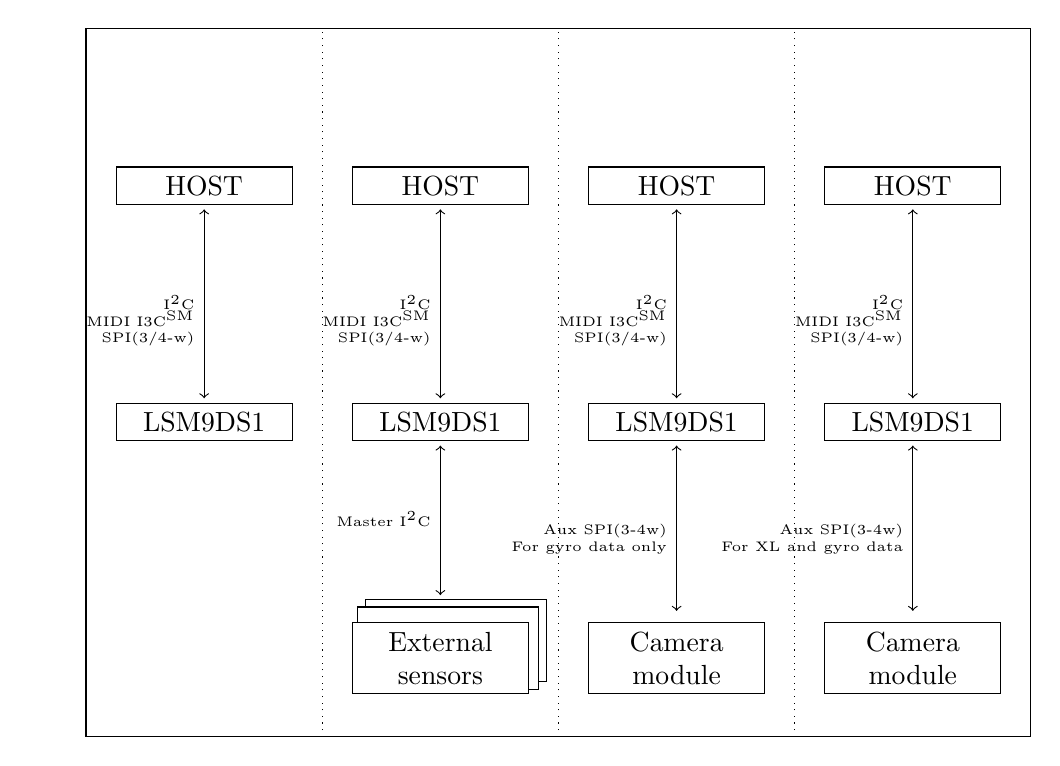
\begin{tikzpicture}
        \draw[fill=white] (0,0) rectangle++(12,9);
        \foreach \x in {3,6,9}{
            \draw[dotted] (\x, 0) -- (\x, 9);}
        \foreach \x in {1.5,4.5,7.5,10.5}{
            \node[draw, fill=white!20, text width=2cm, align=center] at (\x,7) {HOST};
            \node[draw, fill=white!20, text width=2cm, align=center] at (\x,4) {LSM9DS1};}
        \foreach \x in {1.5,4.5,7.5,10.5}{
            \draw[<->](\x,4.3) -- (\x,6.7) node[midway, anchor = mid east, align = right, text width = 2cm, font=\tiny]{I\textsuperscript{2}C\\ MIDI I3C\textsuperscript{SM}\\SPI(3/4-w)};}
        \foreach \x in {7.5,10.5}{
            \node[draw, fill=white!20, text width=2cm, align=center] at (\x,1) {Camera module};
            \draw[<->](\x,1.6) -- (\x,3.7) node[midway, anchor = mid east, align = right, text width = 2cm, font=\tiny]{Aux SPI(3-4w)};}
        \node[anchor=east, align= left, font=\tiny] at (7.5,2.4) {For gyro data only};
        \node[anchor=east,  align= left, font=\tiny] at (10.5,2.4) {For XL and gyro data};
        \draw[fill=white] (3.55,0.7) rectangle++(2.3, 1.05) ;
        \draw[fill=white] (3.45,0.6) rectangle++(2.3, 1.05) ;
        \node[draw, fill=white!20, text width=2cm, align=center] at (4.5,1) {External sensors};
        \draw[<->](4.5,1.8) -- (4.5,3.7) node[midway, anchor = mid east, align = right, text width = 2cm, font=\tiny]{Master I\textsuperscript{2}C};
        
    \end{tikzpicture}
    
    \captionof{figure}{Explication of pin mode}  
\end{center}


\section{Library}

\subsection{Library Description}

To support the project's requirements, we need 3 main libraries, each serving a specific need : 

\begin{enumerate}
    \item \FILE{Wire.h}: This library is a standard Arduino library that facilitates communication between I\textsuperscript{2}C (Inter-Integrated Circuit) devices. I\textsuperscript{2}C is a synchronous serial communication protocol used to connect microcontrollers to external devices. \FILE{Wire.h} provides functions for initializing the I\textsuperscript{2}C bus, sending and receiving data on the bus, and managing multiple devices on the same bus. With this library, developers can easily connect multiple I\textsuperscript{2}C devices, such as sensors or displays, to an Arduino board.
    
    \item \FILE{Kalman.h}: This library implements the Kalman filter algorithm. The Kalman filter is a mathematical technique used to estimate the state of a system from incomplete measurements. It is commonly used in control systems, robotics and navigation applications to improve the accuracy of sensor measurements and reduce errors. \FILE{Kalman.h} provides a simple interface for developers to implement the Kalman filter in their Arduino projects.
    
    \item \FILE{Arduino\_LSM9DS1.h}: The library \FILE{Arduino\_LSM9DS1.h} is a software library designed to facilitate interaction with the sensor accelerometer LSM9DS1, developed by STMicroelectronics. This sensor combines an accelerometer, a gyroscope and a magnetometer in a single package.The library LSM9DS1 provides an interface for accessing the sensor's functionalities, such as reading acceleration, angular velocity and magnetic field data. It can be used to configure various sensor parameters, such as measurement scales, sampling rates and operating modes.
    
    
\end{enumerate}

\subsection{Installation}

The library give some example of sketch, to use this sketch we need to download the library on ArduinoIDE. The library \FILE{Arduino LSM9DS1.h} and \FILE{Kalman.h} can be download directly on Arduino. The library \FILE{wire.h} is used if you imput :  \PYTHON{\#include <wire.h>}

\begin{center}
    \includegraphics[width = 14cm]{Arduino/IMU/wire.png}
    \captionof{figure}{Wire include } 
\end{center}


\begin{center}
    \includegraphics[width = 15cm]{Arduino/IMU/LSM6DSboard.png}
    \captionof{figure}{Board card installation}
\end{center}

\begin{center}	
    \includegraphics[width = 5cm]{Arduino/IMU/LSM9DS1.png}
    \captionof{figure}{Library choice }
\end{center}

\bigskip

\section{Function}

The library LSM9DS1 on Arduino Nano 33 BLE Sense is composed of different function. The function is different if you was on I\textsuperscript{2}C protocol or SPI protocol.

\lstdefinestyle{Arduino}{
    language=Arduino,
    basicstyle=\ttfamily\small,
    keywordstyle=\color{blue},
    stringstyle=\color{yellow!30!black},
    commentstyle=\color{green!60!blue},
    morecomment=[l]{//},
    morecomment=[s]{/*}{*/} }

\subsection{Library \FILE{Wire.h}}


This library is used to devellop communication betwin different composent of Arduino board, it's used for I\textsuperscript{2}C. The library \FILE{Wire.h} is composed by : 
\begin{itemize}
    
    \item \PYTHON{Wire.begin()}: Initializes the library \PYTHON{Wire.h} and prepares the Arduino to act as master or slave on the bus I\textsuperscript{2}C.
    \item \PYTHON{Wire.beginTransmission(address)}: Starts a transmission to a slave device with the specified address.
    \item \PYTHON{Wire.write(data)} : Sends data on the I2C bus during transmission.
    \item \PYTHON{Wire.endTransmission()} : Ends the current transmission and releases the I2C bus.
    \item \PYTHON{Wire.requestFrom(address, quantity)} : Requests data from a slave device with the specified address.
    \item \PYTHON{Wire.available()}: Checks whether data is available to be read after a request.
    \item \PYTHON{Wire.read()}: Reads data received from a slave device.
    
\end{itemize}

We can test the function with on example of the library \FILE{Wire.h}. This is an axemple to test the I\textsuperscript{2}C bus on the board. 
\begin{center}
    
    \captionof{code}{Simple sketch using the sensor LSM9DS1  detection}
    \label{TestWire}
    \ArduinoExternal{}{../../Code/Nano33BLESense/IMU/Test/WireEx.ino}
    
\end{center}
\subsection{Function \PYTHON{IMU.begin()}}


The function to initialized the IMU is \PYTHON{IMU.begin()}, they start the IMU initialization process. This step is important to configures the IMU's basic parameters, set the communications with other devices, and prepares the unit for proper operation. Accurate initialization is essential to ensure the accuracy and reliability of the data provided by the IMU.

An error during the initialization can lead to inaccurate measurements or unpredictable behavior. For example, incorrectly configured measurement parameters or sampling rates can compromise data quality, affecting overall system performance.


\begin{lstlisting}[style= Arduino]
    if (!IMU.begin()) {
        Serial.println("Failed to initialize IMU!");
        while(1){};	}
\end{lstlisting}


\subsection{Function \PYTHON{IMU.end()}} 

This function is composed without parameter. After do this function they return value of 1 if all is good and they return value of 0 if we had some problem.

This function is used to stop or deactivate the IMU once it is no longer required. It frees up the resources used by the IMU and ends its operation cleanly. When called, it ensures that all tasks associated with the IMU are properly finalized, avoiding memory leaks or other problems associated with incomplete de-initialization.

This step helps to ensure the stability and reliability of the system as a whole, by avoiding problems associated with incorrect IMU de-initialization.

The data was return at the end. 

\begin{lstlisting}[style=Arduino]
    if (!IMU.begin()) {
        Serial.println("Failed to initialize IMU!");
        while(1){}; }
\end{lstlisting}


\subsection{Function \PYTHON{IMU.readAcceleration(x,y,z) }}

The \PYTHON{IMU.readAcceleration()} is used to read the IMU accelerometer and obtain the data, this is expressed in gravity (g). This function provides information on the movements detected by the IMU's accelerometer. The resulting acceleration data can be used for a variety of applications, such as shock or motion detection, or inertial navigation. By regularly interrogating the accelerometer and analyzing variations in acceleration, it is possible to understand and react to changes in motion with precision, which is essential in many modern embedded systems and electronic devices.

The parameters x, y and z are floats giving information on the x, y or z-axis 

\begin{lstlisting}[style=Arduino]
    
    float x; 
    float y; 
    float z;
    
    if (IMU.accelerationAvailable()) {
        IMU.readAcceleration(x, y, z);
        
        Serial.print(x);
        Serial.print('\t');
        Serial.print(y);
        Serial.print('\t');
        Serial.println(z);	}
\end{lstlisting}

\subsection{Function \PYTHON{IMU.readGyroscope()}}

Retrieves data from the IMU's gyroscope and returns angular velocity in degrees per second (dps). This function provides information on the rotational movement detected by the IMU's gyroscope. The angular velocity data retrieved can be used in various applications such as robotics, motion tracking or navigation systems. By regularly interrogating the gyroscope and analyzing angular velocity variations, it becomes possible to understand and respond precisely to rotational movements, which is crucial in applications requiring precise orientation control or stabilization.

The parameters x, y and z are floats giving information on the x, y or z axis 

\begin{lstlisting}[style=Arduino]
    float x, y, z;
    
    if (IMU.gyroscopeAvailable()) {
        IMU.readGyroscope(x, y, z);
        
        Serial.print(x);
        Serial.print('\t');
        Serial.print(y);
        Serial.print('\t');
        Serial.println(z);	}
\end{lstlisting}



\subsection{Function \PYTHON{IMU.accelerationAvailable()}}

This function allows you to check the status of IMU acceleration data, indicating whether or not new data is ready to be retrieved.

In scenarios such as motion tracking, robotics or navigation systems, where the IMU continuously captures acceleration data, the availability of new data determines the system answers. Test the IMU at regular intervals is used for application and they can check for acceleration currently or non, ensuring that the system remains synchronized with object movements in real time.

When the function returns a value of 1, this means that new acceleration data is available, enabling the system to extract the data and process it further. A value of 0 indicates that there have been no recent acceleration updates.

\begin{lstlisting}[style=Arduino]
    float x, y, z;
    
    if (IMU.accelerationAvailable()) {
        IMU.readAcceleration(x, y, z);
        
        Serial.print(x);
        Serial.print('\t');
        Serial.print(y);
        Serial.print('\t');
        Serial.println(z); }
    
\end{lstlisting}


\subsection{Function \PYTHON{IMU.gyroscopeAvailable()}}

This function ask if new gyro data are available for the IMU and they returns a value 0 if no new gyro data is available, and 1 if new gyro data is ready to be retrieved.

In applications requiring real-time monitoring of rotational motion, such as drone stabilization, virtual reality systems or inertial navigation, the system can determine whether to wait for updated gyroscope readings or proceed to process available data.

A value of 1 indicates that new gyro data is available, enabling the system to retrieve and use this information for adapted the orientation tracking or motion control. Conversely, a feedback value of 0 indicates that there have been no recent updates to the gyroscope measurements, prompting the system to wait for new data to become available before proceeding.

\begin{lstlisting}[style=Arduino]
    float x, y, z;
    
    if (IMU.gyroscopeAvailable()) {
        IMU.readGyroscope(x, y, z);
        
        Serial.print(x);
        Serial.print('t');
        Serial.print(y);
        Serial.print(' t');
        Serial.println(z); }
\end{lstlisting}


\subsection{Function \PYTHON{IMU.accelerationSampleRate()}}

This function is designed to provide information on the sampling rate of the IMU's accelerometer. The function \PYTHON{IMU.accelerationSampleRate()} returns the accelerometer sampling rate, expressed in Hertz (Hz). This value represents the frequency at which the accelerometer takes measurements and provides acceleration data. It indicates how many times per second the accelerometer registers changes in acceleration along its axes.

In activities such as motion tracking, gesture recognition or vibration analysis, knowledge of the accelerometer's sampling rate ensures that the system can accurately capture and respond to changes in motion dynamics. 

\begin{lstlisting}[style=Arduino]
    Serial.print("Accelerometer sample rate = ");
    Serial.print(IMU.accelerationSampleRate());
    Serial.println(" Hz");
    Serial.println();
    Serial.println("Acceleration in g's");
    Serial.println("X \t Y  \t Z");
\end{lstlisting}



\subsection{Function \PYTHON{IMU.gyroscopeSampleRate()}}

To recover and communicate the specific rate at which the gyroscope, integrated into the inertial measurement unit (IMU), collects data samples. This frequency is usually expressed in hertz (Hz), corresponding to the number of samples acquired per second. This is the frequency at which the gyroscope takes measurements, giving an idea of its operational efficiency and performance.

\begin{lstlisting}[style=Arduino]
    Serial.print("Gyroscope sample rate = ");
    Serial.print(IMU.gyroscopeSampleRate());
    Serial.println(" Hz");
    Serial.println();
    Serial.println("Angular speed in degrees/second");
    Serial.println("X tY tZ");
    
\end{lstlisting}

